\section{Introduction}

Electronic currency has a long and seemingly fruitless history until recently with the emergence of Satoshi's Bitcoin \cite{btc-whitepaper}. % in 2008.
 The Blockchain, the essence of electronic cryptocurrency, is poised to disrupt many domains including the financial industry, internet of things (IoT), energy, healthcare, utilities, and insurance to name a few.
%In the last few
 Blockchain gets its name from the consensus protocol of electronic currency that mediates transactions, and establishes a universally agreed upon transaction history. %,
%While electronic currency can trace its roots back to the 1980s with proposals and ideas from Chaum's untraceable payments \cite{chaum}, B-money \cite{B-money}, Hashcash \cite{hashcash}, and Digicash \cite{digicash}, and many more.
%Many of these proposals had novel implementations incorporated in the system however none of them were able to succeed in the market.
%Each of the aforementioned variants focused on a core component to modern cryptocurrencies such as privacy, decentralization, security, etc.
%Bitcoin was the first successful implementation that had these secure components realized.
% 
 This document proposes Blockchain support for existing traditional financial derivatives as well as crypto derivatives.
More abstractly, it addresses the following problem: How can we integrate existing financial markets into the cryptocurrency ecosystem? % a way?
%
%While there are many projects addressing this issue, many of them focus on the exchange of assets or facilitating the adoption of cryptocurrencty as a payment method for goods and services.
%
Specifically we propose a decentralized derivative exchange with support for contracts on traditional commodities through immutable programmable smart contracts on the Blockchain.
Additionally, the exchange aims to support a new age of Blockchain securities built on top of cryptocurrency tokens of which can bleed the lines between stock and currency.
 Our Blockchain based platform leverages the advantages of the cryptographically secure Blockchain, purely transparent financial contracts, and the decentralized nature of the Blockchain, and applies them to traditional financial derivatives markets. 
 The advantage of a Blockchain based exchange can be expressed in reduced fees due to programmable smart contracts, increased transparency through the universal public ledger that Blockchain offers making the ABCDE's orderbook completely public and auditable and facilitates. 
 Additionally the turing-complete smart contract programming language reduces counterparty risk while the ABCDE is able to perform the same functions as traditional exchange components. %through our platform. 

 \section{Motivation}
 We are proposing a Blockchain derivative exchange based in the cryptocurrency and Blockchain ecosystem with the following motivation.
\begin{itemize}
%\item Create an exchange for financial derivatives in the cryptocurrency ecosystem
\item Maximize financial transparency and immutability.
\item Financial decentralization
\item Programmable automatic derivative contracts to reduce middlemen payments 
\item Cross-chain (cryptocurrency independent) order matching to maximize exchange volume
%\item Reduce middlemen payments through decentralization
\end{itemize}

\section{Components}
\begin{itemize}
  \item User interface
  \item Contract setup
  \item Orders matching contract
  \item External data source contract
  \item Clearinghouse contract
\end{itemize}

Figure \ref{overview} illustrates the interaction at a high level of the system components.
The following sections go into details of the listed components.

\begin{figure*}
  \centering
  %\label{overview}
  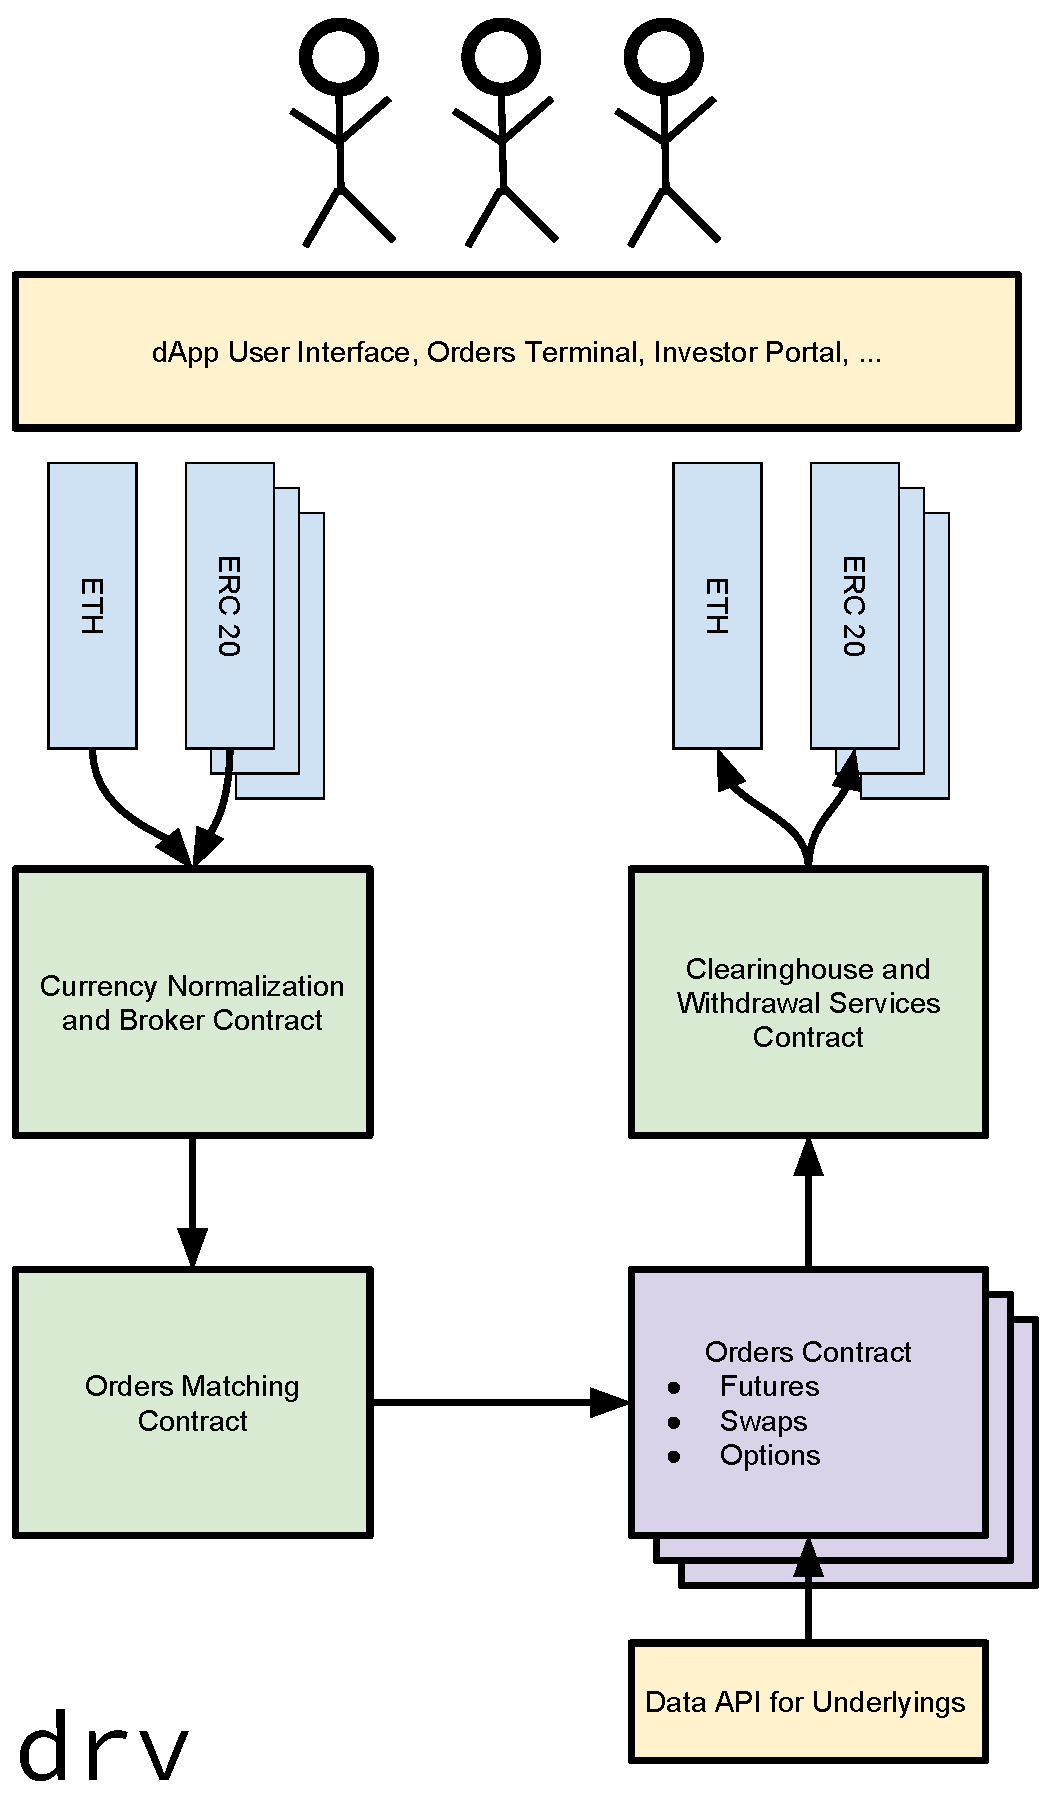
\includegraphics[scale=.5]{Overview.pdf}
  \caption{The core components of ABCDE.}
  \label{overview}
\end{figure*}

\subsection{User Interface}
The user interface for BCDE will have the following components:
\begin{itemize}
  \item Registration: required for legal purposes
  \item Trader Terminal: will display information regarding derivative types, prices, volumes, etc.
  \item Investor Portal: the point of contact for ICO backers
\end{itemize}

A common misperception of Blockchain is its use for illicit behavior. 
However Public-Private key infrastructure, the underlying technology for Blockchain identities, is also widely used for authentication such as in PGP or internet certificates.
In order to comply with regulations and restrictions ABCDE will utilize Know Your Customer (KYC), Anti-money Laundering (AML), and Counter-Terrorism Financing (CTF) through Cynopsis-Solutions.
A registration process will enable us to authenticate users allowing us to comply with any regional regulations.

Additionally, perhaps the most important component for a trader is a terminal that would allow a user to place orders, and see information such as trade volume.
The terminal would also provide a way for traders and investors to manage and settle their existing positions.
The trader terminal provides the trader information on how to convert between currencies during contract settlement and creation which can add utility.


Finally, in order to maximize transparency of the exchange, an investor portal will allow the public to view and audit company operations, business directions, and request features.


\subsection{Contract Setup}
Because there are an ever expanding construction of new Blockchain services and tokens, and a large variety of popular cryptocurrencies% and tokens
, all underlying contracts are done with Ethereum. %DRV tokens as described in Section \ref{DRV}.
%The major benefit of constructing all contracts in DRV is that this creates a single orderbook thereby increasing the total volume on the exchange.
%Thus, externally a trader or investor can buy a contract using various currencies including even DRV and get matched with a seller using a different cryptocurrency.
%Contracts are listed in multiple popular cryptocurrencies, i.e., Bitcoin, Ethereum, and other popular ERC20 tokens. 
%Internally, there is a transfer to DRV tokens to maximize volume on the exchange. 
%This transfer is done decentralized and cryptographically secure across chains using atomic swaps \cite{atomic-swaps}. 
%Additionally this requires the derivative exchange to include currency exchange functionality.
%The cryptocurrencies that are supported depends on their ability to be cross chain compatable.
%Any currency or token that support atomic swaps, Bitcoin, Bitcoin Cash, Ethereum, Decred, Litecoin, and any token built on the Ethereum that supports the ERC20 specification.

\subsection{Order Matching}
All underlying derivative contracts are created with DRV tokens, thus orders are easier to match as there would be greater trade volume when compared to a separate order book for each currency.
The implementation of the order matching contract is centralized, however the  matching is done on top of the Ethereum blockchain which makes the verification process of the contract decentralized.
Thus, the Blockchain can enforce transparency, immutability, fairness, and auditability properties which motivates our design of ABCDE.
Additionally, all fees for matching are actually given(required) to the Blockchain miners which verify the previously mentioned properties.

\subsection{External Data Source Contract}
\label{oracle}
In order to settle a contract and to complete the margin changes, the spot price of the underlying asset is required.
For both traditional derivatives and crypto derivatives, there will be a spot price required.
%\subsubsection{Connecting the Blockchain to Off-chain Data}
%While there are many industries interested in the decentralized nature of the Blockchain there still exists many challenges.
%Going back to the example of a financial derivative on the Blockchain, if Alice wants to buy a futures contract on Apple (AAPL) but not on the New York Stock Exchange (NYSE), then her profit flow would be determined by the market price of AAPL on the Blockchain.
%Alice interfaces with a Blockchain smart contract and not the NYSE, however AAPL's price while public is not on the Blockchain.
Therefore the smart contract will need to have a connection to the data source an existing stock exchange or a cryptocurrency exchange in the latter case.

There also exists many other uses for integrating off-chain data into the Blockchain.
For example, automatic insurance payouts in the case of natural disasters, connection IoT device actuation, and prediction markets such as Augur \cite{Augur} \cite{Truthcoin}, and Gnosis \cite{Gnosis} to name a few.
Therefore this is not a new problem and there exists multiple solutions we can leverage.

The main challenge is then how to trust someone to inject these values into various smart contracts.
\textit{Oracles} are a name given for the party or service that is trusted to introduce external data into the Blockchain.
The idea of a centralized trusted party is contrary to Blockchain however.
There has been various work recently on solutions.
One such proposal is called ChainLink \cite{ChainLink} which is a decentralized oracle service.
However even if a oracle service is distributed and decentralized there remains the challenge of trust in the service.
Additionally the complexity associated with ChainLink increases the fees required.
Another service, Oracalize \cite{Oracalize} is a centralized data service that provides the ability to run authenticity proofs which the service can offload the trust to well-known and widely used services such as intel SGX, Android and Google's SafetyNet, Qualcomm's TEE, Amazons TLS Notery, and more.
The authenticity can also be proven on the Blockchain which would allow the existing decentralized infrastructure to validate the authenticity and correctness of the input data.
Since the data validation is critically important in financial contracts the design of our system revolves around verifying the data.

%\

%TODO: ADD infor about data sources both crypto and trad, try to figure out which authenticity proof to use.


\subsection{Clearinghouse Contract}
\label{clearinghouse}

While traditional financial clearing houses operate between two parties engaged in a contract for facilitating payments and reducing counterparty risk, our smart contract based system progmatically enforces counterparty payment which in turn reduces risk for .

While a centralized counterparty clearing is still needed in out platform, its roll transitions to picking up one end of the transaction if a party defaults on a margin call since all derivatives are marked to market daily.

\

TODO Does this reduces the need for centralized counterparty clearing. Or maybe just the risk? %or...?  

%\section{DRV Token}
%\label{DRV}\label{drv}

%\ 

%\section{Research Direction}
%This document discusses the existing state of Blockchain technology and overviews some financial securities.
%The research proposed can be expressed in the following points:
%
%\begin{itemize}
%\item Implementation of cryptocurrency financial derivatives and integration into Blockchain.
%\item Implementation of existing financial derivatives found on traditional markets into the Blockchain environment.
%\item Implementation of Blockchain models in a discrete event simulator for planning and evaluation of existing and future Blockchain protocols and contracts.
%\end{itemize}

%\subsection{Crypto Derivatives}
%A basic building block for the realization of cryptocurrency derivatives is atomic transfers as introduced earlier.
%Crypto Derivatives are currency derivatives similar to fiat currencies seen in existing financial markets.
%They differ from their fiat counterparts however because their implementation is purely decentralized by means of Blockchain technology.
%One of the main challenges of crypto derivatives are cross chain smart contracts.
%This is the first point of investigation because it has the lowest barrier to entry.

%\subsection{Integration of Existing Financial Instruments on the Blockchain}
%In section \ref{oracle}, a couple of challenges were discussed with obtaining off-chain data into smart contracts.
%While existing solutions rely on trusted third parties, it is desired to reduce the trust requirements in line with the cryptocurrency philosophy.
%Therefore we need to investigate the requirements of external data sources and use cryptographic protocols to ensure integrity and accountability and most desirably a trusted smart contract system.
%This step will essentially integrate off-chain data for contracts that have physical real-world data sources.


\pagebreak

\

\section{Summary}
\if 0
\subsection{Roadmap}

\begin{itemize}
  \item Q3 2018
    \begin{itemize}
      \item ERC20 Contract for DRV
      \item Testnet implementation of futures contracts
      \item ICO launch
    \end{itemize}
  \item Q4 2018
    \begin{itemize}
      \item User interface alpha release
      \item Order Matching Contract for DRV
      \item Clearinghouse and settlement contract for DRV
    \end{itemize}
  \item Q1 2019
    \begin{itemize}
      \item Legal filings
      \item Main-net alpha release
      \item Atomic swaps for crypto currency independent contracts (testnet)
      \item Expansion of derivative contract options (testnet)
    \end{itemize}
  \item and Beyond
    \begin{itemize}
      \item Refine user interface
      \item Full deployment to main-net
    \end{itemize}
\end{itemize}

\fi

\subsection{Conclusion}
This proposal highlights the research challenges of integrating financial derivatives into a Blockchain based system and provides motivation for such integration.
It also overviews the existing state of connecting external data into the Blockchain, as well as connecting Blockchains together for more robust intracurrency exchange.
The proposed research direction can be summarized as follows: investigation into cross-Blockchain contracts for the creation of a Intra-Blockchain currency market, the integration of off-chain data into the Blockchain to create transactions that utilize external data sources, and the modeling of proposed research problems and solutions through simulation.


\pagebreak
